%%%%%%%%%%%%%%%%%%%%%%%%%%%%%%%%%%%%%%%%%%%%%%%%%%%
%
%  New template code for TAMU Theses and Dissertations starting Fall 2012.  
%  For more info about this template or the 
%  TAMU LaTeX User's Group, see http://www.howdy.me/.
%
%  Author: Wendy Lynn Turner 
%	 Version 1.0 
%  Last updated 8/5/2012
%
%%%%%%%%%%%%%%%%%%%%%%%%%%%%%%%%%%%%%%%%%%%%%%%%%%%
%%%%%%%%%%%%%%%%%%%%%%%%%%%%%%%%%%%%%%%%%%%%%%%%%%%%%%%%%%%%%%%%%%%%%%
%%                           SECTION V
%%%%%%%%%%%%%%%%%%%%%%%%%%%%%%%%%%%%%%%%%%%%%%%%%%%%%%%%%%%%%%%%%%%%%

\chapter{\uppercase{Experiment \& Results}}

\label{sec:results}



\section{Dataset Combination \& Feature Selection}
\label{Datacombination}

In order to apply machine learning algorithm to forecast bike rental demand effectively, important features from the datasets (City bike trip data, Weather data, Holiday data) needs to be collected. From the target dataset mentioned earlier in this thesis, the common fields like `year', `month', `day', `hour' counted once. Alsothose bike data contains more than $3$million rental data, male data is about 2,342,359 and female data is about 651,398 and rest is unknown gender data. These bike rental data is then combined with the weather and holiday data as shown in Table~\ref{datacombo}. `Feature no.' field shows the number of features related to the second column which is the name of the feature. Then Table~\ref{datacombo} also shows the type of the features (numeric or binary), source of the features (1= city bike trip data, 2= weather data, 3= holiday data) and the combined hours means the hour numbers combined together to build the dataset. For example, 1-8 feature is about the hourly rental count, which is a numeric data, for combined hours field hour -1 is the previous hour data, -24 is the data from 24 hours earlier and so on. 



\begin{table}[]
\centering
\caption{Feature selection}
\label{datacombo}
\begin{tabular}{||l|l|l|l|l||}
\hline
Feature no. & Name                  & Type    & Combined hours                      & Source \\ \hline \hline
1-8         & Hourly rental count   & numeric & -1,-24,-48,-72,-96,-120,-144,-168 & 1      \\ \hline
9-16       & Age                   & numeric & -1,-24,-48,-72,-96,-120,-144,-168 & 1      \\ \hline
17-24       & Trip duration         & numeric & -1,-24,-48,-72,-96,-120,-144,-168 & 1      \\ \hline
25-32       & Bike count            & numeric & -1,-24,-48,-72,-96,-120,-144,-168 & 1      \\ \hline
33-40       & Month                 & numeric & -1,-24,-48,-72,-96,-120,-144,-168 & 1      \\ \hline
41-48       & Day                   & numeric & -1,-24,-48,-72,-96,-120,-144,-168 & 1      \\ \hline
49-56       & Snow depth            & numeric & -1,-24,-48,-72,-96,-120,-144,-168 & 2      \\ \hline
57-64       & Snow fall             & numeric & -1,-24,-48,-72,-96,-120,-144,-168 & 2      \\ \hline
65-72      & Wind speed            & numeric & -1,-24,-48,-72,-96,-120,-144,-168 & 2      \\ \hline
73-80       & Temperature          & numeric & -1,-24,-48,-72,-96,-120,-144,-168 & 2      \\ \hline
81-88       & Precipitation         & numeric & -1,-24,-48,-72,-96,-120,-144,-168 & 2      \\ \hline
89-96     & Holiday               & binary  & -1,-24,-48,-72,-96,-120,-144,-168 & 3      \\ \hline
97-104     & Weekday               & binary  & -1,-24,-48,-72,-96,-120,-144,-168 & 3      \\ \hline
105-112    & Weekend (not holiday) & binary  & -1,-24,-48,-72,-96,-120,-144,-168 & 3      \\ \hline
\end{tabular}
\end{table}


\section {Baseline Algorithms}
\label{BaseAlgos}

In order to compare the results of proposed method some baseline models are chosen. These are- Linear regression, Neural network, Support vector regression (SVR) which are very popular and very effective machine learning algorithms in recent time. A brief description about this algorithms are given below in order to understand the methods better and how it compares to our model. 

\subsection{Linear Regression}
\label{LR}

Regression is  one of the most widely used models in recent years according to ~\cite{seber2012linear}. This algorithm assumes that the target variable $y$ on features $x_1,x_2,x_3 ... x_n$ is linear, thus it tries to find the best suitable model to fit the target. This model is then used to do prediction ~\cite {han2011data}. 

\begin{figure}
\centering
\begin{adjustbox}{addcode={\begin{minipage}{\width}}
{\caption{Simple Linear Regression~\cite{wang2016forecasting}}  
\label{linear}
\end{minipage}}}
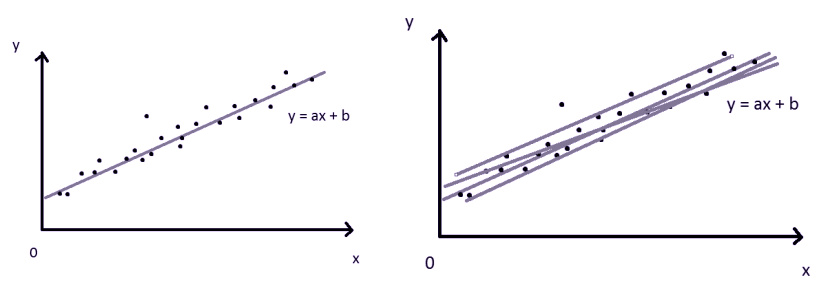
\includegraphics[scale=0.4]{figures/linear.png}
\end{adjustbox}
\end{figure}

From the figure~\ref{linear} we can see a simple example of linear regression. For two variable $x  \&  y$ and the relationship between them is $y=ax+b$. From this example at any given value of $x$, dependent variable $y$  can be predicted . But many lines can fit the model perfectly, for which residuals should be taken into count. Suppose if,  $A(x_1,y_1)$ using $y=ax+b$ can predict $A^\prime(x_1,ax_1+b) $ then the disparity between $A$ and $A^\prime$ is called residual ~\cite{montgomery2012wiley}. The residual sum of squares, $ RSS = (y_1-ax_1-b)^2 +(y_2 - ax_2 - b )^2 + ... + (y_n-ax_n-b)^2)$ [figure~\ref{linear2}].


\begin{figure}
\centering
\begin{adjustbox}{addcode={\begin{minipage}{\width}}
{\caption{Residual example~\cite{wang2016forecasting}}  
\label{linear2}
\end{minipage}}}
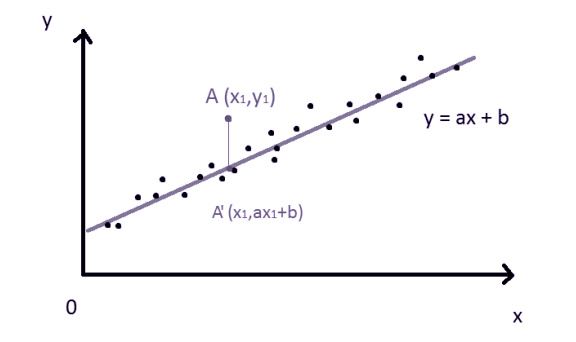
\includegraphics[scale=0.4]{figures/linear2.png}
\end{adjustbox}
\end{figure}



\subsection{Neural Network}
\label{NN}

Neural network is currently one of the most discussed and most commonly used machine learning algorithm. It is getting more and more attention from the researchers all over the world~\cite{rojas2013neural}. Its methodology is based on animal neurons, with a joined assembly of simple elements. The internal connection strengths ensures the processing ability of the network or weights which is obtained through learning~\cite{gurney1997introduction}. 

According to~\cite{rojas2013neural} an abstract neuron [figure~\ref{NN1}] can have $n$ inputs. Each input frequency t can convey $x_t$ information, weight $w_t$ and $f$ being the primitive function. The transmitted information is integrated at the neuron and the primitive function is then evaluated~\cite{rojas2013neural}.

\begin{figure}
\centering
\begin{adjustbox}{addcode={\begin{minipage}{\width}}
{\caption{Abstract neuron~\cite{rojas2013neural}}  
\label{NN1}
\end{minipage}}}
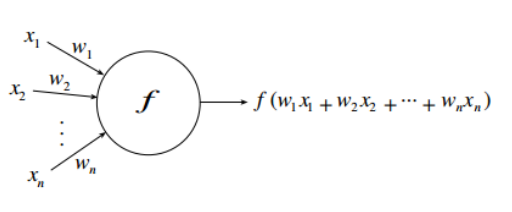
\includegraphics[scale=1.2]{figures/NN1.png}
\end{adjustbox}
\end{figure}


Neural network has the ability to combine $n$ basic functions. In figure~\ref{NN2} four functions $f_1,  f_2, f_3, f_4$, network function  $ \Phi $  is estimated at the point $x, y, z$. Weights $ \alpha_1, \alpha_2,… \alpha_5 $ can also create different network functions.





\begin{figure}
\centering
\begin{adjustbox}{addcode={\begin{minipage}{\width}}
{\caption{Functional model of a Neural Network~\cite{rojas2013neural}}  
\label{NN2}
\end{minipage}}}
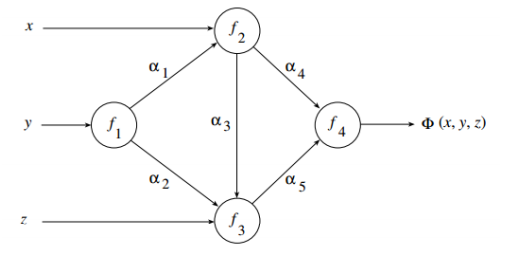
\includegraphics[scale=1.2]{figures/NN2.png}
\end{adjustbox}
\end{figure}

\subsection{Support Vector Regression}
\label{SVR}

Support vector machine (SVM) is a very powerful and widespread supervised machine learning model~\cite{friedman2001elements} which are used to solve regression or classification problems. The version of it that deals with regression is known as Support Vector Regression (SVR). SVR is commonly known for its high level of generalization, therefore, this model can be used in new, previously unobserved data with high accuracy. In SVR figure~\ref{NN2}, support vectors fabricated on the $\epsilon$ tube bounding decision shell, called training samples. Residuals which are fewer than $\epsilon$ has no influence on predictions.

\begin{figure}
\centering
\begin{adjustbox}{addcode={\begin{minipage}{\width}}
{\caption{Non-linear SVR ~\cite {jain2014forecasting}  }  
\label{SVR}
\end{minipage}}}
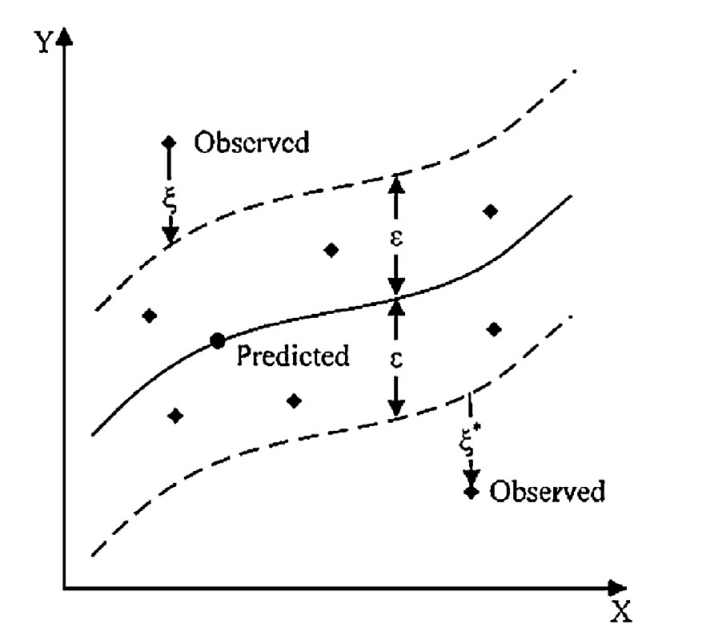
\includegraphics[scale=0.7]{figures/SVR.png}
\end{adjustbox}
\end{figure}


Suppose, for a given dataset ${(X_i, Y_i)}^{i=N} _{i=1}$, where input variables X and output Y, SVR estimates the relationship as : 

$Y - W.\Phi (X)+b$ , here $\Phi (X)$ is a non-linear kernel function which non-linearly maps from the input space X to the feature space. By minimizing the following function coefficients W and b are determined :


$min  {\frac{1}{2}}\parallel w\parallel ^{2} + C\frac{1}{N}\sum_{i=1}^{N}\xi _i+\xi _i^*$

with constraints –


$Y_i - W.\Phi (X_{i})-b\leq \epsilon +\xi _{i}$

$W.\Phi (X_{i})+b-Y_{i}\leq \epsilon +\xi _{i}^*$

$\xi ,\xi _{i}^*\leq0$

Here, to attain acceptable results $W$ the weight should be as flat as achievable. $\xi _{i}$ $ \xi _{i}^*$ are the residuals beyond $\epsilon $ and the regularization parameter is the cost $C$. 




\section{Evaluation Metrices}
\label{Evaluation}

In order to assess the model accuracy, this work uses four evaluation metrices. Mean absolute percentage of error (MAPE), Root-mean-square error (RMSE), normalized Mean absolute error (NMAE), and Normalized root-mean-square error (NRMSE). 

MAPE metric has been used in a amount of prediction studies~\cite{ hu2015mid}~\cite{edwards2012predicting}. It describes the average absolute error as percentage by the following equation-

$MAPE = \frac{1}{N}\sum^{N}_{i=1}(\left | \frac{y_i - \hat y_i}{y_i} \right |\times 100)$

Here, $y_i$ is the actual value,  $ \hat y_i $ is the predicted value and $N$ being the number of observations. The value of MAPE relies on the score and the lower the score is higher the performance is. MAPE value for lower forecast can not exceed $100 \%$, but there is no limit for higher forecasts.  MAPE can also not be used if there are zero values as it will be divided by zero. 

RMSE depends on the measure of the variables and should be used to compare forecasting for the similar series across the models as relative measure. Similar to MAPE, the smaller the error better the forecasting. 

$RMSE = \sqrt[]{\frac{1}{N}\sum_{i=1}^{N}(\hat y_i - y_i)^2}$

One issue with evaluating with RMSE is the forecast error varies across time. Non- linearity in the model or deviations in exogenous variables can cause this issue. According to~\cite{fair1990comparing} no severe statistical analysis can be put on the RMSE because they are not approximations of any factor in the model. 


NMAE measure normalizes the mean absolute error by the range of possible data values. NMAE is defined as follows- 


$ NMAE=\frac{\sum_{i=1}^{N}(\left |  \hat y_i-y_i\right |)}{\sum_{i=1}^{N}(\left |  y_i\right |)}$

NRMSE is the normalized root mean square error which compares between models with different scales. Similar to RMSE the value is expressed as percentage and lower value means less residual differences. 

$  NRMSE=\sqrt[]{\frac{\sum_{i=1}^{N}(  \hat y_i-y_i)^2}{\sum_{i=1}^{N}(  y_i)^2} }$ \\

%\subsection{Tensorflow}
%\label{Tensorflow}
%
%For implementing the Convolutional Neural Network, Tensorflow- an open source software for the numerical computation using data flow graphs is used ~\cite{tensorflow}. In Tensorflow the nodes represents the mathematical operations and graph edges represents the tensors (multi dimensional data arrays) between them. The advantages of using Tensorflow is to apply computation to one or more CPU’s or GPU’s with a single API. 




\section {Results}
\label {results}


This section focuses on how the proposed CNN model is actually performing against the three baseline models (Linear regression, Neural Network, SVR). As mentioned earlier Table~\ref{datacombo} we selected the features from those three datasets and created the time series featureset. The featureset contains $9\times14$, total $126$ features which has current hour data as well as 8 previous hours data based on the Table~\ref{datacombo}. Two different training and testing dataset were created based on monthly bike rental demand records. These dataset counts are also shown in Table~\ref{dataset}.  Proposed model CNN is used from Tensorflow with the parameter estimation of AdomOptimizer, filter $3\times 3 $, max pooling size $2 \times 2$.  

%%%%

\begin{table}[]
\centering
\caption{Dataset counts}
\label{dataset}
\begin{tabular}{||c|l||c|l||}
\hline
\multicolumn{2}{||c||}{Training set}                     & \multicolumn{2}{c||}{Testing set} \\ \hline \hline
\multicolumn{1}{||l|}{Male} & Female                    & Male  & Female                   \\ \hline
3612                       & \multicolumn{1}{c||}{3529} & 720   & \multicolumn{1}{c||}{714} \\ \hline
\end{tabular}
\end{table}

%%%%



\section {Discussion}
\label {Discussion}

From the results in Table~\ref{femalecomp} and Table~\ref{malecomp} we can see the comparison between methods for forecasting bike rental demand for both female and male. Comparing CNN with other methods for both genders shows that CNN outperforms other baseline models with significant advantages constantly in all four different metrices. It also shows that results gained from the male datasets are far superior than the result gained from female datasets. MAPE results gained for female varies from 8-12 \% for baseline models where CNN shows 7 \%. It also shows better percentage level for male dataset where CNN is only 3-4 \%. The reason for male data to show better forecasting results is because there are a lot of data available for male users as shown in the figure~\ref{genderpie}. As the results from those two table showing CNN is performing better than the baseline models it is understandable that the goal of the thesis and the methodology used to achieve this, is proving to be effective. 

Even though CNN results are better than baseline models it is still confusing to decide which structure of CNN should be used. For female dataset 5 layer CNN is working better than others where in male dataset 7 layer CNN is working better. In overall, treating this bike rental data as an image processing sample and doing demand forecasting of hourly rental bike demand using CNN is a successful demand forecasting technique. 

% Please add the following required packages to your document preamble:
% \usepackage{multirow}
\begin{table}[]
\centering
\caption{Comparison of results between proposed and baseline models (Female dataset)}
\label{femalecomp}
\begin{tabular}{|c|c|c|c|c|}
\hline
\multirow{2}{*}{Model Name} & \multicolumn{4}{c|}{Dataset Used - Female}                                                                              \\ \cline{2-5} 
                            & \multicolumn{1}{l|}{MAPE} & \multicolumn{1}{l|}{NMAE} & \multicolumn{1}{l|}{RMSE} & \multicolumn{1}{l|}{NRMSE} \\ \hline
Linear Regression            & 8.987                     & 0.062                     & 0.509                     & 0.084                      \\ \hline
Neural Network              & 11.263                    & 0.084                     & 0.677                     & 0.112                      \\ \hline
SVR                         & 8.869                     & 0.084                     & 0.052                     & 0.085                      \\ \hline
5 Layer CNN                 & \textbf{7.373}            & 0.051                     & \textbf{0.327}            & \textbf{0.045}             \\ \hline
6 Layer CNN                 & 7.654                     & \textbf{0.050}            & 0.043                     & 0.073                      \\ \hline
7 Layer CNN                 & 7.489                     & \textbf{0.050}            & 0.425                     & 0.070                      \\ \hline
\end{tabular}
\end{table}

%%%%
\begin{table}[]
\centering
\vspace{1ex}
\caption{Comparison of results between proposed and baseline models (Male dataset)}
\label{malecomp}
\begin{tabular}{|c|c|c|c|c|}
\hline
\multirow{2}{*}{Model Name} & \multicolumn{4}{c|}{Dataset Used - Male}                                                                       \\ \cline{2-5} 
                            & \multicolumn{1}{l|}{MAPE} & \multicolumn{1}{l|}{NMAE} & \multicolumn{1}{l|}{RMSE} & \multicolumn{1}{l|}{NRMSE} \\ \hline
Linear Regression            & 4.330                     & 0.038                     & 0.378                     & 0.052                      \\ \hline
Neural Network              & 6.068                     & 0.053                     & 0.548                     & 0.075                      \\ \hline
SVR                         & 4.529                     & 0.039                     & 0.408                     & 0.056                      \\ \hline
5 Layer CNN                 & 4.059                     & 0.036                     & 0.361                     & 0.049                      \\ \hline
6 Layer CNN                 & 4.031                     & 0.036                     & 0.347                     & 0.048                      \\ \hline
7 Layer CNN                 & \textbf{3.531}            & \textbf{0.030}            & \textbf{0.327}            & \textbf{0.045}             \\ \hline
\end{tabular}
\end{table}

%%%%%%%%%%%%%%%%%%%



